\documentclass[11pt]{article}
\usepackage{graphicx}  	% Lets you install pictures
\usepackage{amssymb}    % Cool Math symbols
\usepackage{hyperref}	% clickable hyperlinks
\usepackage{fullpage}

\begin{document}

\title{Introduction to Linux}
%\author{Erica Caden}
%\date{}

\maketitle
All of this is identical for any unix operating system, i.e.~Ubuntu, Fedora, MacOS, Scientific Linux, etc.
\begin{itemize}
\item terminal: shell from which you navigate around the directory structure
%
%
\item pwd: present working directory
\item mkdir: create a directory
\item cd: change directory\\ \texttt{\$ cd -} returns you to the directory you were previously in
\item ls: list items in a directory. \\Many options available, -l(ong), -a(ll), -t(ime ordered), -h(uman readable), -r(everse order)
\item $\sim$: home directory \\ \texttt{\$ cd $\sim$} brings you to your home directory
\item clear: clear the terminal screen
\item cp: copy file
\item mv: move/rename file
\item rm/rmdir: remove a file/directory \\ rm doesn't ask for permission, and can't be undone. Be absotively posilutely sure you want to \textbf{permanently} delete something.
\item man: look at the manual for a command 
\item more: displays file to screen, one page/line at a time.
\item less: displays file to screen, one page/line at a time,  clears screen when finished. 
\item head: writes first 10 lines of a file to the screen
\item tail: writes last 10 lines of a file to the screen
\item grep: searches for a string inside a file or files\\ \texttt{\$ grep "string" file\_pattern}
\item find: finds files \\ \texttt{\$ find -iname "MyCProgram.c"}
\item cat: prints to screen, combines files into one
\item echo: prints a string to the terminal
\begin{itemize}
\item $>$ : redirect/overwrite output in file
\item $>>$ : append output to existing file
\item $|$ : pipe the output of a command to a file 
\end{itemize}
\item sudo: super user do, for installing or running certain higher level commands
\item apt-get/yum/homebrew: search for/install packages 
\item ps: list the processes running. end process with  (kill -9) 
\item sudo: Run command as the super user, requires root account password
\item diff: look at the differences between two files, additions, deletions\\\texttt{\$ diff my\_file.txt my\_file\_new.txt}
\item ssh: Secure Shell, use to log into remote machines \\ \texttt{\$ ssh -X myname@science1.snolab.ca}
\item scp: Secure CoPy, transferring files between local and remote machines \\ \texttt{\$ scp my\_local\_file.txt myname@science1.snolab.ca:. }
\item tar: creates and manipulates streaming archive files
\begin{itemize}
\item create: -czvf archivefile.tar dir\_to\_tar/ (Create a Zipped File, Verbosely) 
\item extract: -xzvf archivefile.tar (eXtract from a Zipped File, Verbosely)
\end{itemize}
\end{itemize}
\begin{figure} [hb]
\centering
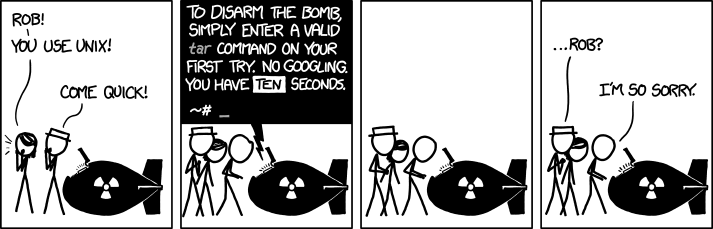
\includegraphics[width=\textwidth]{tar.png}
\caption{tar, from \texttt{www.xkcd.com/1168}}
\end{figure}
\end{document}
